\chapter{Описание метаязыка QReal} \label{appendixB}

\begin{center}
	\begin{longtabu} {| X[1 l m] | X[1.6 c m] | X[3 m] |}
		\caption{Метаязык системы QReal} \\
		\tabucline-
		Название                    & Внешний вид                                                                     & Описание \\
		\tabucline-
		\endfirsthead
		\tabucline-
		Название                    & Внешний вид                                                                     & Описание \\
		\tabucline-
		\endhead
		\noalign{\vspace{3mm}}\caption{Метаязык системы QReal (многостраничная)} \\
		\endfoot
		\everyrow{\tabucline-}
		Metamodel Diagram           & 
\includegraphics[scale=1]{part4/metalanguage/metamodelDiagram.png}              & Корневой элемент метамодели. Может содержать в себе 
		                                                                                                                узлы Meta Editor Diagram (метамодели языков, входящих в 
		                                                                                                                плагин), свойства этого элемента содержат настройки сборки 
		                                                                                                                редактора, такие как относительный путь к исходным файлам 
		                                                                                                                QReal. \\
		Meta Editor Diagram         & 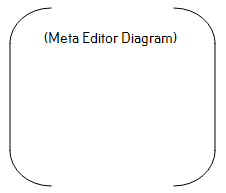
\includegraphics[scale=0.5]{part4/metalanguage/metaEditorDiagram.png}           & Корневой узел метамодели одного визуального языка. Может 
		                                                                                                                содержать в себе узлы Node, Edge, Enum. Для каждого узла 
		                                                                                                                этого типа в метамодели редактора будет сгенерирована своя 
		                                                                                                                вкладка в палитре элементов. \\
		Package Diagram             & 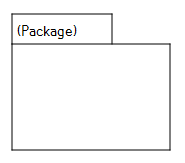
\includegraphics[scale=0.7]{part4/metalanguage/packageDiagram.png}              & Пакет. Предназначен для группировки метамоделей и обеспечения переиспользования 
		                                                                                                                фрагментов метамоделей. Также может быть корневым элементом метамодели. Может  
		                                                                                                                содержать в себе другие пакеты или узлы Metamodel Diagram. На данный момент  
		                                                                                                                функциональность этого узла поддерживается лишь частично и используется в основном для 
		                                                                                                                визуализации зависимостей по включению между метамоделями при импорте их из XML-описаний. \\
		Node                        & 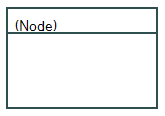
\includegraphics[scale=0.7]{part4/metalanguage/node.png}                        & Представляет узел создаваемого языка. Может содержать в себе узлы Property, Possible Edge, 
		                                                                                                                Properties as Container. Свойства включают в себя имя узла, отображаемое имя узла (с 
		                                                                                                                первым работают генераторы и другие инструменты, отображаемое имя показывается 
		                                                                                                                пользователю), форму узла (форма хранится в виде XML-строки, для её редактирования из 
		                                                                                                                метаредактора открывается редактор формы фигур), некоторые свойства, связанные с 
		                                                                                                                пользовательским интерфейсом (текст всплывающей подсказки для этого узла, может 
		                                                                                                                ли узел менять размер, можно ли создавать вложенные в него узлы с помощью контекстного меню). \\
		Property                    & 
\includegraphics[scale=0.7]{part4/metalanguage/property.png}                    & Свойство. Не имеет какого-либо специального графического оформления, может находиться 
		                                                                                                                только внутри узлов Node и Edge. Для свойства возможно указание имени, отображаемого имени, 
		                                                                                                                типа, значения по умолчанию. Типом свойства может быть один из элементарных типов 
		                                                                                                                (целочисленный, булевый, строковый), тип-перечисление, определённый в этой же
		                                                                                                                метамодели, или ссылочный тип, указывающий на объект типа, определённого в этой же метамодели. \\
		Possible Edge               & 
\includegraphics[scale=0.7]{part4/metalanguage/possibleEdge.png}                & Возможная связь. Указывает, какие элементы мгут быть соединены связью. Задаются имя 
		                                                                                                                узла, из которого может начинаться связь и имя узла, в котором связь может заканчиваться, 
		                                                                                                                также есть возможность указать, направленная связь или нет (то есть можно или нет поменять 
		                                                                                                                начальный и конечый узлы местами). Может находиться внутри узла Node. \\
		Properties as Container     & 
\includegraphics[scale=0.7]{part4/metalanguage/propertiesAsContainer.png}       & Свойства контейнера. Этот элемент отвечает за задание чисто визуальных свойств 
		                                                                                                                взаимодействия узла с вложенными в него узлами, например, должен ли узел  
		                                                                                                                автоматически располагать вложенные узлы друго под другом в столбик, или пользователь 
		                                                                                                                может произвольно располагать вложенные узлы внутри узла-контейнера. Также можно задать 
		                                                                                                                расстояние между вложенными элементами и расстояние от элементов до границы 
		                                                                                                                контейнера, если контейнер сам отвечает за расположение вложенных узлов. Можно указать, 
		                                                                                                                должен ли контейнер автоматически сжиматься или расширяться в соответствии со своим содержимым. \\
		Edge                        & 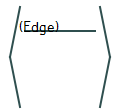
\includegraphics[scale=0.7]{part4/metalanguage/edge.png}                        & Связь. Задаётся имя, отображаемое имя связи, тип линии (сплошная, пунктирная и т.д.), текст, 
		                                                                                                                отображаемый на линии (либо фиксированный, либо свойство связи из репозитория). Кроме  
		                                                                                                                того, связь может иметь свойства, так же как узел. Также можно указать, из какого типа портов 
		                                                                                                                связь может исходить и в какой тип портов связь может входить (см. описание элемента Port). 
		                                                                                                                Если типы портов не указаны, связь может быть подключена к любому порту, если он относится к 
		                                                                                                                допустимому узлу (см. описание элемента Possible Edge). \\
		Association                 & 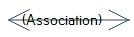
\includegraphics[scale=0.7]{part4/metalanguage/association.png}                 & Элемент для задания свойств начала и конца связи, вкладывается в элемент Edge. Для конца 
		                                                                                                                связи можно указать имя конца и тип стрелки (открытая, закрытая, закрашенная стрелка, 
		                                                                                                                закрашенный и незакрашенный ромб, без стрелки). \\
		Enum                        & 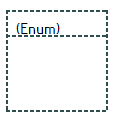
\includegraphics[scale=0.7]{part4/metalanguage/enum.png}                        & Тип-перечисление. Позволяет указать фиксированный набор значений, который можно 
		                                                                                                                использовать как тип какого-либо свойства. Состоит из набора элементов Value. \\
		Value                       & 
\includegraphics[scale=0.7]{part4/metalanguage/value.png}                       & Одно значение типа-перечисления, вкладывается в элемент Enum. Содержит 
		                                                                                                                только имя значения. \\
		Port                        & 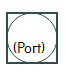
\includegraphics[scale=0.7]{part4/metalanguage/port.png}                        & Объявление типа порта, к которому могут быть подключены определённые связи. При 
		                                                                                                                редактировании формы узла имеется возможность для каждого порта, рисуемого на  
		                                                                                                                изображении узла, указать его тип, а для связи указать тип порта, к которому связь может быть 
		                                                                                                                подключена. \\
		Import                      & 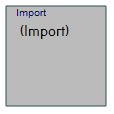
\includegraphics[scale=0.7]{part4/metalanguage/import.png}                      & Импорт элемента. Позволяет использовать элементы одной метамодели в другой 
		                                                                                                                метамодели. Имеется возможность переопределить имя элемента и его  
		                                                                                                                отображаемое имя. \\
		Container                   & 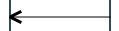
\includegraphics[scale=0.7]{part4/metalanguage/container.png}                   & Связь, задающая допустимую вложенность между элементами. Направлена от элемента, 
		                                                                                                                который может вкладываться в другой, к тому элементу, в который он может вкладываться. По  
		                                                                                                                умолчанию элементы не вкладываются друг в друга. Связь учитывает отношение 
		                                                                                                                наследования, то есть любой потомок вкладываемого элемента может быть вложен в 
		                                                                                                                любой потомок элемента, в который исходный элемент вкладывается. Этим отношением могут 
		                                                                                                                быть связаны только узлы. \\
		Explodes To                 & 
\includegraphics[scale=0.7]{part4/metalanguage/explodesTo.png}                  & Эксплозия, или отноошение раскрытия. Связывает элемент и тот элемент, в который 
		                                                                                                                первый элемент может раскрываться (например, узел, обозначающий подпрограмму, и диаграмму  
		                                                                                                                подпрограммы, в которую он раскрывается). Связь содержит ряд вспомогательных свойств, 
		                                                                                                                например, необходимо ли немедленно создать тот узел, на который ссылается исходный, или 
		                                                                                                                сделать ли связь переиспользуемой (в этом случае узел, соединённый этой связью, 
		                                                                                                                добавляется на пользовательскую палитру и может быть добавлен в других местах 
		                                                                                                                диаграммы или на другие диаграммы, с сохранением связи-раскрытия). Связь также  
		                                                                                                                учитывает отношение наследования. \\
		Inheritance                 & 
\includegraphics[scale=0.7]{part4/metalanguage/inheritance.png}                 & Наследование. Обозначает, что один элемент является подвидом другого элемента и может 
		                                                                                                                быть использован везде вместо своего предка. Наследование означает, что узел-потомок имеет  
		                                                                                                                все свойства узла-предка, а также наследует все отношения вложенности и раскрытия, 
		                                                                                                                которыми был связан предок. Наследование может быть множественным.
		\label{tab:metalanguage}
	\end{longtabu}
\end{center}